\documentclass[conference]{IEEEtran}
\usepackage{graphicx}
\usepackage{multicol, blindtext}

\ifCLASSINFOpdf
\else
\fi
\hyphenation{}

\begin{document}

\newcommand{\comment}[1]{{}}

%\setcounter{secnumdepth}{3}

\newcommand{\figh}[3]
{
\begin{figure}
%\centerline{\includegraphics[height=#2]{fig/#1.pdf}}
%\centerline{\includegraphics[height=#2]{fig/#1.eps}}
\centerline{\includegraphics[height=#2]{fig/#1.jpg}}
\caption{\label{fig:#1} #3}
%\vspace{-0.1in}
\end{figure}
}

\newcommand{\figw}[3]
{
\begin{figure}
%\centerline{\includegraphics[width=#2]{fig/#1.pdf}}
%\centerline{\includegraphics[width=#2]{fig/#1.eps}}
\centerline{\includegraphics[width=#2]{fig/#1.jpg}}
\vspace{-0.1in}
\caption{\label{fig:#1} #3}
\vspace{-0.1in}
\end{figure}
}

\newcommand{\figwtwocol}[3]
{
\begin{figure*}
%\centerline{\includegraphics[width=#2]{fig/#1.pdf}}
%\centerline{\includegraphics[width=#2]{fig/#1.eps}}
\centerline{\includegraphics[width=#2]{fig/#1.jpg}}
\vspace{-0.1in}
\caption{\label{fig:#1} #3}
\vspace{-0.1in}
\end{figure*}
}

\newcommand{\minifigw}[2]
{
\includegraphics[width=#2]{fig/#1.pdf}
%\centerline{\includegraphics[width=#2]{fig/#1.eps}}
}

\newcommand{\figwh}[4]
{
\begin{figure}
%\centerline{\includegraphics[height=#2]{fig/#1.pdf}}
%\centerline{\includegraphics[height=#2]{fig/#1.eps}}
\centerline{\includegraphics[width=#2,height=#3]{fig/#1.jpg}}
\caption{\label{fig:#1} #4}
%\vspace{-0.1in}
\end{figure}
}


\title{Mesos, Swarm, Kubernetes, Fleet and ECS: \\
A Comparative Study of Container Orchestration Tools}
 \author{
  \IEEEauthorblockN{Piush K. Sinha, July 2016
  }
}


% make the title area
\maketitle


\begin{abstract}
This paper presents an overview of container orchestration tools and its basic features. In the paper, we have discussed the architecture and various features of Apache's Mesos, Google's Kubernetes, Docker's Swarm, CoreOS's Fleet and Amazon's ECS followed by their comparison. We have also discussed related open issues and proposed our approach to solve them.
\end{abstract}

\IEEEpeerreviewmaketitle

\section{Background}
\label{sec:bg}

\subsection{Isolation and Resource Utilization}
Every application~\cite{turtles} comes with software and hardware requirements which is necessary to run those applications. In the following section, we have discussed the idea of isolating these dependencies with a better resource control. It is implemented by using a traditional processes in an operating system while virtual machines are used in case of hypervisors. Our goal is to have a more dynamic and flexible implementation of the isolation and resource control.
\subsection{About isolation and resource sharing in VMs}
\label{sec:irsVM}
In hypervisor based virtualization, isolation is achieved by having related process grouped together in virtual machines (VMs). Each of these VMs have its own operating system, its own virtualized physical memory, virtual CPU(s) and virtual input/output devices. Processes running in one VM is totally unaware of the processes running in other VMs. Although complete isolation is achieved, but having its own operating system and the abstraction provided by the hypervisor make the system virtualization too heavy and slow which affects the overall performance.

\subsection{About isolation and resource sharing in traditional process}
\label{sec:irsTP}
Traditional processes running directly on host operating system have much better performance compared to the processes running in VMs, though they don't provide complete isolation. Although traditional processes have their own virtual address space and their own access to host's services using system calls, they share too much including file system, storage, network and all the  I/O devices.

\subsection{Best of both: Container based virtualization}
\label{sec:bob}
Using operating-system level virtualization, also called as container based virtualization, we can achieve better performance than hypervisor based virtualization and more isolation than traditional processes. Using the host's operating system kernel, container based virtualization provides multiple isolated execution environments in userspace. (openvz-intro reference). Chroot, freeBSD JAIL, cgroups and namespace are the techniques used to implement container based virtualization.

\begin{enumerate}
\item Chroot and freeBSD JAIL: 
Container based virtualization technique follows the concept of containing a process, also known as jailing a process, using chroot. 'chroot' allows the calling process and its child processes to be isolated by changing its root directory to a given path(sans ref). However this isolation is restricted only to the file system and doesn't include isolation of process space and network space (kamp ref).
FreeBSD Jail is another technique that provides jailing a process which is built on 'chroot'. In addition to limiting the access to the file system, Jails protects rest of the system from the jailed process by virtualizing the network subsystem and the set of users, including its own root user (kamp ref).
\item cgroups and namespace:
Linux cgroups and linux namespace has changed the concept of container based virtualization by introducing linux containers (lxc). Instead of virtualizing the entire machine, linux namespace allows virtualizing a part of it. It enables different processes to have different view of the system making the whole linux container look like as a system of its own (Multiple Instances Eric ref). However, namespace itself do not provide resource management (namespace paper). Linux containers uses cgroups to limit the resources to a process or a group of processes (cgroup online kernel ref).
\end{enumerate}

\subsection{Isolation and resource sharing in distributed system using containers:}
\label{sec:IsRsDCcont}
A distributed system is a cluster of multiple machines where the resources of the machines are shared and used as one single large machine. A cluster of containers uses containers to create and deliver the applications, mostly one application in one container. Thus, the resources are divided among the containers as per their resource requirements. Due to being launched inside containers, applications are totally unaware of each other making them totally isolated. Although concept of container has been present for a long time (since the early time of UNIX), there has been a recent surge in use of containerized applications in distributed system by companies providing cloud services. In a production environment, the number of the containerized applications becomes enormously large. This creates the need of an orchestration tool that can control and manage the containers running in a distributed system.

In the following section, we have discussed about container orchestration tool and its basic features. In the remaining paper, we have discussed five specific container orchestration tools in detail and compared their features. At the end of the paper, we have talked about the open issues related to resource sharing and isolation in a distributed system that uses containers. We have provided our approach to solve those issues and discussed how to implement it.


\section{Container Orchestration Tool}
\label{sec:ContainerOrchestrationTool}
It is a group of machines that runs and manage the containerized applications. These machines could be physical machines or virtual machines. The software tool that manages it is called container orchestration tool. 

Usually, one of the cluster machines is chosen as the master and rest of the machines act like workers. The master machine basically does scheduling of the applications and deploy it using a container on the one of the worker machines. A worker machine executes the scheduled application using containers. This is the basic architecture of a container orchestration tool.

The basic features of a container orchestration tool are:
\begin{enumerate}
\item Microservices:
Master machine breaks down a monolithic application into smaller parts in such a way that these parts are manageable individually. Breaking down into smaller parts allows to scale them horizontally. thus, an application is a collection of smaller services called as microservices. These microservices implement one function of the application. This feature allows to have clear interfaces between these smaller parts which ultimately help in scaling up the applications.

\item Service discovery:
As mentioned above, microservices have clear itnerfaces that allows to communicate with each other. These microservices need to be discovered in order to be used by other services or applications. Container orchestration tool uses a naming resolution service to discover the services and to resolve the requested services to its target. Some of the container orchestration tools use labels for the service discovery.

\item Scheduling: Tbe master machine in container orchestration tool should be able to package up the job in a container and decide on which worker machine this job should be sent. 

Scheduling is a totally dynamic process which is based on the requirements and availability of the resources across the cluster. To do scheduling, the master machine uses the information of the availability of free hardware resources (e.g. memory, disk space, CPU, etc)on every worker machine and availability of some special hardwares(e.g. GPUs) as well.

Scheduling also involves having multiple instances of a task and distributing it across the multiple machines. Scheduling multiple instances of a task helps in achieving fault tolerance.

Scheduling should be totally dynamic. What it means is that scheduling should reschedule the tasks depending upon the state of the cluster.

Sometimes a scheduler is also required to schedule correlated tasks on same machine.

\item High Availability of manager node: In a cluster, one of the nodes can be chosen as the manager node. Its task is to coordinate with the worker nodes and the containers running on those nodes. Failure of manager node will shut down the whole cluster. To avoid this scenario, it is important to have a cluster which can recover from the failure of the manager node.


\item  Horizontal scaling/recovery from container failure: A container orchestration tool should have a provision for scaling up the application horizontally i.e. having multiple instances of a container. This feature allows to have zero downtime in case of container failure.

It is possible that a container running on a node can fail while it is still executing the task. Additionally node failure will also cause all the containers to fail. It is important to automatically restart work of a container from its failed state on healthy nodes.

Recovering from a container failure using multiple instances may require some kind of failover mechanism e.g. load balancing technique.

\item  High utilization and efficiency rates: ????????needs more clear explanation????????
 Google was able to dramatically increase resource utilization and efficiency after moving to containers.


\item Easy to upgrade: A container orchestration tool that is up on a running cluster must not go down while upgrading the versions of its components which might be time consuming. An upgrade should also allow to rollback to previous version to revert the changes. 


\item Easy to manage and monitor: Although a container orchestration tool provides cluster management and monitoring, a good orchestration tool should make the cluster management easy/automated by doing most of the task by itself. 

\end{enumerate}



In the following sections, we have discussed the container management tools listed below:
\begin{itemize}
\item Apache's Mesos
\item Google's Kubernetes
\item Docker's Swarm
\item CoreOs's Fleet
\item Amazon's EC2 Container Service (ECS)
\end{itemize}
We have given an overview of each of the above mentioned tools and have discussed their features. We have also done a comparative study of their features.


\section{Apache Mesos:}
\label{sec:mesos}

\figwtwocol{elastic_sharing}{5in}{Elastic Sharing Mesos}

Mesos was started in 2009 to try and increase the performance and utilization of clusters. The project's key idea was to have a framework for the distributed system so that  the nodes in a cluster can be used as a shared pool instead of statically partitioning each of those individual nodes (filip). 

Usually in a static sharing or static partitioning, one server runs on one node availing all its resources. Most of the times, the resources on such nodes are wasted as the server doesn't utilize all the resources of the node. Using the elastic sharing, Mesos layer of abstraction talks to all the available nodes in the cluster aggregating the resources, making a cluster of nodes look like as one single machine.

As shown in Figure~\ref{fig:elastic_sharing}, ....
%\begin{figure*}
%\centering
%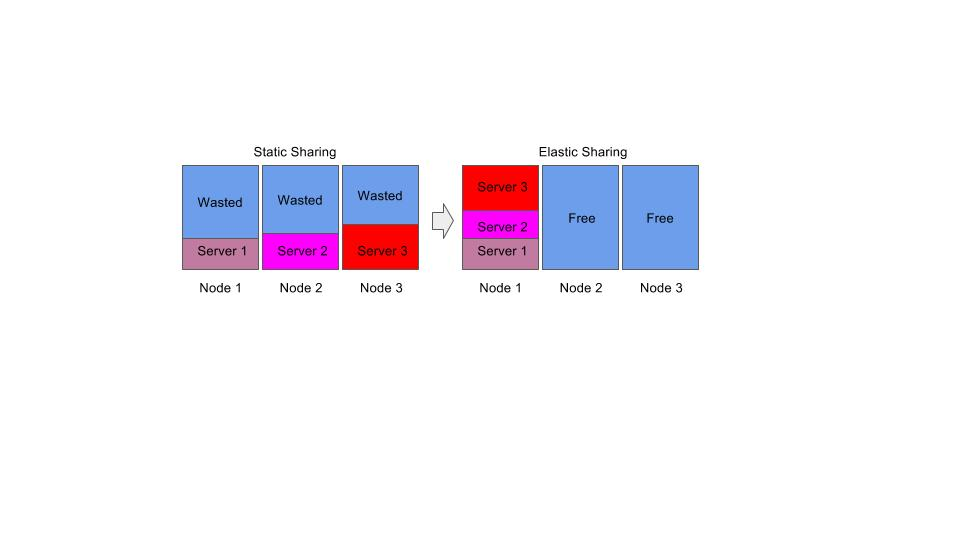
\includegraphics{./fig/elastic_sharing}
%\label{fig:elastic_sharing}
%\end{figure*}


\figw{mesos}{3.4in}{Apache's Mesos Architecture}
As shown in Figure~\ref{fig:mesos}, Mesos architecture consists of master nodes and agent nodes, framework and Zookeeper. In Mesos cluster, Master nodes run the master process that manages the slave processes running on agent nodes. Slave processes run the tasks, for e.g. a database query or bash command, which are scheduled to be executed on the agent nodes. 

Framework is a Mesos application which has has two component: scheduler and executor. Using their scheduler, framework schedules the task to run on the agent nodes. The tasks are executed by executor process that is launched on each agent nodes. Before scheduling a task, framework needs to be registered with the master node. The services running on the top of the Mesos framework don't care about the cluster resources. The services/frameworks running on top of the Mesos requests to the Mesos layer for the resources required at that particular time.

Master node offers the available resources on the agent nodes to the registered framework. These offered resources are the list of free resources on the agent nodes. Master node gets the information about the available resources from the agent nodes and it decides how many resources to be offered to frameworks. Master node makes this offer by having the nearest approximation of the available resources which matches the framework's request. Master node only offers the available resources to the registered frameworks.
 
After receiving the offer, the framework, e.g. Marathon or Hadoop, chooses to accept or reject the offer. It can reject the current offer and wait for the offer which satisfies their request. If the offer is accepted then the framework deploys the task on the agent node. Once the task is completed, the resources are freed up by the master node. 

Zookeeper is a tool which is used provide the high availability of the master nodes in Mesos. It replicates the master nodes and coordinate with them. One of these masters is selected as the leader.


Following are the features of Mesos:

\begin{enumerate}
\item High Availability: Mesos provides high availability of master node by having multiple replicas of the master node. It uses Zookeeper tool to replicate the master node and coordinate between these replicas. However, Mesos doesn't provide fault tolerance for the application failure. It only detects the failure, but doesn't handle it.

\item Linear Scalability: Mesos framework is easily scalable to tens of thousand nodes.

\item Resource Isolation: Using Linux containers, Mesos provides performance isolation between tasks of different frameworks on the same agent node.

\item Fault Tolerance: In case of node failure, Mesos notifies the framework about the node failure and its executor. Depending ontheir policies, the framework acts on those notifications.

In Mesos, frameworks are allowed to have multiple schedulers to be registered with master node. In case one of the scheduler fails, the Mesos master will notify the another scheduler to take over. Sharing the state between the schedulers is upto the frameworks.

\item Cross Platform support: Mesos can run on different platform like Linux, Windows and OSX.

\item Two level scheduling: Using the resource offer technique, Mesos separates the resource management and process scheduling.  Mesos master decides about the resources to be offered to the frameworks, while frameworks decides how to manage their distributed processes. Frameworks uses short tasks and elastic resource utilization to improve the response time of the tasks.

\item HTTP APIS: Mesos provides HTTP APIs to monitor and operate cluster and to develop new distributed applications.
WEB UI

\end{enumerate}




















\section{Google's Kubernetes:}
\label{sec:kubernetes}
Google's Kubernetes is an open source container orchestration tool which is built on the experience of 15 years of running production workloads at large scale. As a container management framework, it deploys containerized application using Docker containers and provides application scaling, scheduling of containers, routing of traffic, load balancing and container monitoring. 

Kubernetes implements the master-slave architecture. In Kubernetes cluster, one node works as the Kubernetes Master node which is responsible for coordinating with other nodes called as worker nodes. Worker nodes are the nodes in the cluster which actually runs the requested applications using containers. Each of these worker nodes runs an agent process, called kubelet, which talks to master node.

Master node runs a scheduler service. The scheduler service is used to monitor the resources and the workload on the worker nodes. Based on the available resources, it schedules the applications in a container on a node in the cluster. 

Containerized applications are not deployed directly on the nodes. They are assigned to pods. Pods are the basic unit on a worker node which represents related containers grouped together. Pods are basically a group of containers which act as a single application.

\begin{figure*}
\centering
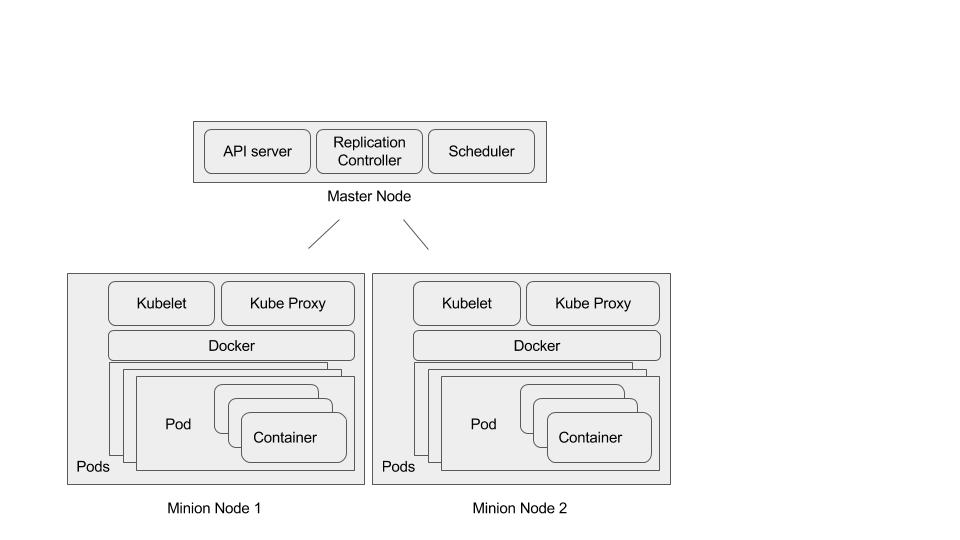
\includegraphics[scale=0.5]{./fig/kubernetes}
\caption{Google Kubertnetes Architecture}
\label{fig:kubernetesArch}
\end{figure*}

Following are the features of Kubernetes:

\begin{enumerate}
\item Pods:
A container is launched inside the smallest deployable unit called pods. One single pod can run multiple containers in it. These containers in one single pod share the network namepsace and pod's IP address. Each Pod has their own IP addresses. However, pod's network space is flat i.e. they don't need NAT to communicate with each other.

\item Service:
A group of pods having the same functionalities are called service. They run an application as a service which is used by other applications without knowing its lower details. The pods in a  service are associated and discovered using the labels (explained below). Load balancer, one of the services of Kubernetes, balances the workload among the associated pods. If one of the pods having too much workload, then load-balancing service will use kube-proxy to balance the workload. Kube-proxy will forward it to any of the less loaded pods in the same service. Kube-proxy are the network proxy that runs on every worker nodes.

\item Labels:
Pods can be labeled using a key/value data. This labels are user-defined tags on the pods. Labeling is not limited to the pods. A service running in Kubernetes can also be labeled. 

\item Replication Controller:
Pods can be replicated to provide availability using replication controller running on the master node. The replication controller replicates the pods using the pod template. It also maintains the pod's replicas using the labels tagged on the related pods. If one of them dies, replication controller will create another pod using the template. Replication controller can also scale down the pods. 

\item Volumes:
Since the containers are ephemeral, it is needed to recover the files residing on the failed container to restart it from its failed state. Kubernetes achieve this by supporting the concept of volumes. volume is an abstraction type which is basically a directory at the core level. The volume lives as long as the pod is alive and the data in the volume is maintained even if a container fails.

\item ETCD and state management:
Etcd is a service running on the master node which is used to store the configuration data in key/value pair distributed over the cluster. It is used state management and service discovery. 

\item API server:
Kubernetes provides users an API server running on master node to configure workloads and containers. API server is based on RESTful interface allowing different tools and packages to communicate with the master node.

\item Automated rollouts and rollbacks:
Any changes in the application will be rolled out without killing the instances of the application. If anything goes wrong, then Kubernetes will rollback to the old state.

\end{enumerate}
\section{Docker's Swarm:}
\label{sec:swarm}
Docker Swarm is Docker’s native clustering tool that allows to make a group of Docker engines into a single, virtual Docker Engine. This allows the services to scale out as if they are running on a single machine with large resources. Swarm allows to get rid of the trouble of deciding the nodes where to start the docker containers. Although docker swarm is a clustering tool, but the definition of cluster is limited to the pool of Docker engines. 

\begin{figure*}
\centering
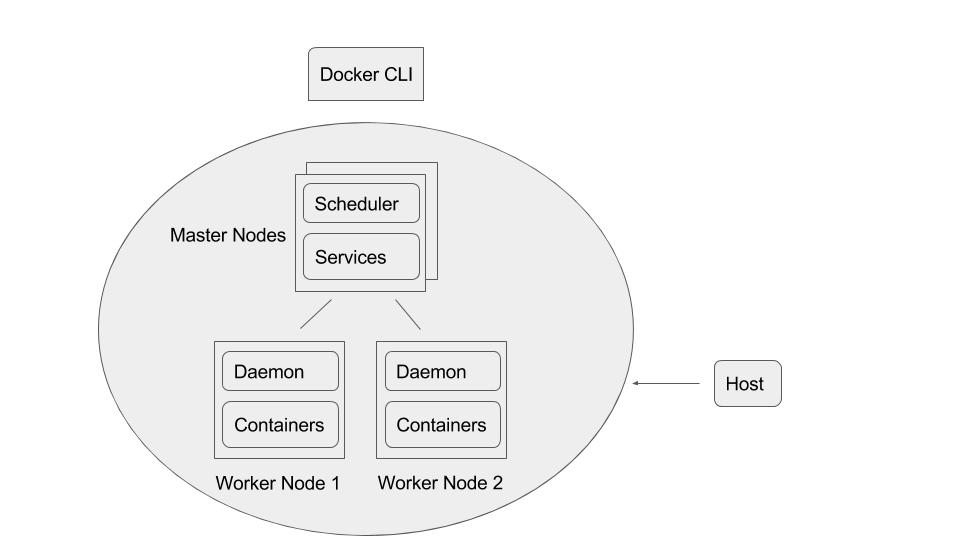
\includegraphics[scale=0.5]{./fig/swarm}
\caption{Docker Swarm Architecture}
\label{fig:swarmArch}
\end{figure*}

To create a swarm of Docker’s engine, it first requires steps of
\begin{itemize}
\item defining the cluster,
\item joining of hosts to the cluster and,
\item creating the cluster manager. 
\end{itemize}
Hosts become nodes after they join the swarm. These nodes are classified as manager nodes and worker nodes in Swarm. Manager nodes are responsible for the scheduling, coordination and managing the resources of swarm nodes.

Worker node’s job is to run the tasks which are forwarded by the manager node to them. By default, all manager nodes are worker nodes. Docker Swarm selects one of these  manager nodes as primary that manages the swarm, does scheduling and launches the tasks to a worker node in container. 

Following are the features of Swarm:
\begin{enumerate}
\item Compatibility with Docker APIs:
Swarm uses the standard Docker APIs. This allows any services or applications, which were using Dockers, to scale out to multiple nodes. Swarm’s use of Docker’s API make it easy to use. However, this makes Swarm to inherit the constraint of Docker’s APIs. 

\item High availability:
High availability in swarm is achieved by having multiple instances of the manager node. The primary manager talks to the nodes of the cluster. If the primary manager fails, one of the other instance of the manager node will replace it and will become the primary manager node.

\item Pluggable schedulers:
Although swarm has its own scheduler, but it is optional. Swarm allows to use third party schedulers like Mesos by using the plugin while running the tasks using Docker clients.  This follows the Docker philosophy of “batteries included but removable.”

\item Node Labeling:
One of the most powerful features of swarm is labeling of the nodes. Like Kubernetes, Swarm allows the users to put custom label in the nodes. The labeling of nodes allows the users to constrain which nodes a container can start on. Swarm also allows to tag a node with multiple labels. This allows the user to put more broad constraints on a container.

\item Container Affinity:
In some cases, the placement of a container must be relative to other containers. Swarm lets you define those relationships through affinities. Affinities are automatically generated when the relationship between containers is implied.

\item Swarm Discovery:
Swarm can use hosted discovery service, static file, etcd, consul or zookeeper for the service discovery.

\item TLS:
TLS authentication can be enabled to secure the communication to and from Swarm.

\item Integrated networking and Volumes:
Since Swarm is a Docker’s native tool, it can use Docker Networking, Volumes and plugins through their respective Docker commands.


\item Flexible Scheduling:
In addition to labeling and affinity features, multiple scheduling strategies like spread and binpack gives the flexibility to assign the container to a specific node maximizing the resource utilization.


\item High Scalability:
In production environment, Swarm’s performance has been tested up to 50000 containers without any performance drop. 

\end{enumerate}
\section{coreOS:}
\label{sec:fleet}
CoreOS is a cluster-wide operating system to manage and run containers. It is a lightweight linux distribution which doesn't have any package manager. CoreOS uses docker containers to run its applications. It is platform independent which means coreOS can run on bare metal, virtual machine, cloud or cloud and physical machine together (coreOS website).

\begin{figure*}
\centering
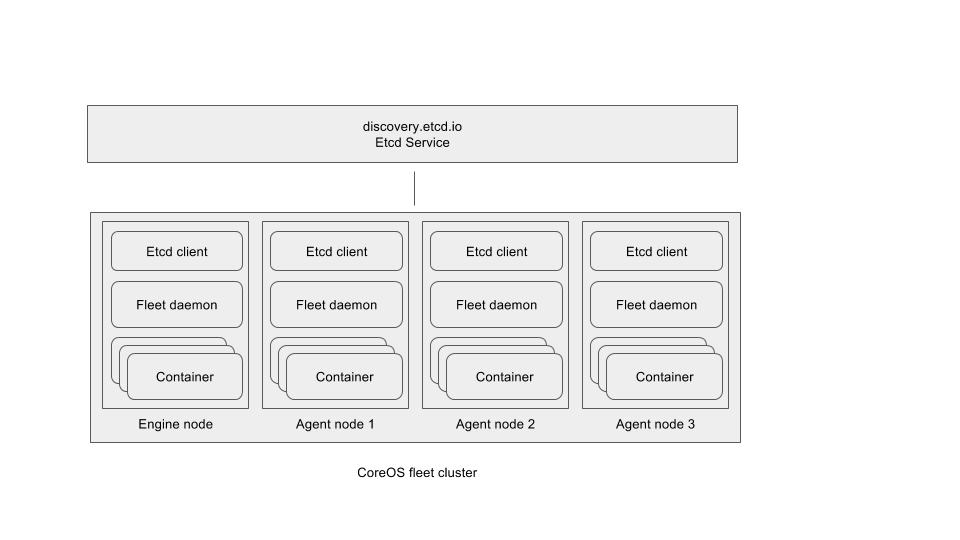
\includegraphics[scale=0.5]{./fig/fleet}
\caption{CoreOS Fleet Architecture}
\label{fig:fleetArch}
\end{figure*}

\begin{enumerate}
\item Fleet:
CoreOS's Fleet is the cluster manager which is built on systemd. Systemd, an init system, is a project separate than CoreOS which resolves the issues with sysV init and allows process management during boot-up. While systemd is for single machine, coreOS's Fleet is for the whole cluster. Fleet uses systemd unit files extended with some additional Fleet parameters to run any task. The systemd unit file are the configuration files which has the information about the task which Fleet uses to decide where to run the task. Fleet extends systemd feature to start, stop and monitor the units. Fleet can run two types of units: One is standard unit and other is global unit. Standard units are the tasks that run on a single node and it can be rescheduled on a new node if the node dies. Global units are the tasks that keep running cluster-wide i.e. on all the nodes. Global units are mainly used for services.
CoreOS has one fleet daemon running on each of the nodes on the cluster. Once the cluster is up, one of these fleet daemon is chosen as the master called engine and rest of the daemons are called agents. The engine daemon schedules the tasks dynamically monitoring the changes in the cluster. Engine process identifies the nodes to run the units and then forwards the tasks to that identified node to process it. This is done by agent process which keeps running on each of the nodes. The agent daemon keeps updating the status of the task back to the engine daemon. 

Following are the features of Fleet:

\item Etcd:
Etcd is a service that runs on every nodes. Its instance running on every machine needs to be synchronized and connected to build a cluster. Its job is more than just to coordinate between engine and agents daemons. It is used to store the key/value data for the whole cluster. It contains all the information about units, continuous updates about their states, configuration and nodes. Etcd is a stored in distributed manner over the cluster which makes it safe from the single node failure. 

\item Fault Tolerance:
The communication between engine and agents are done by using etcd tool. If any of the node fails while running the task, the agent daemon fails to update the status back to the engine. The engine understands that the node has failed and it reschedules the task on a new node. This self healing architecture of Fleet provides fault tolerance for each of the node. 

\item High Availability:
Fleet allows to run multiple instances of services on different nodes making it highly available.

\item Service Discovery:
Since the Etcd is distributed, any change in configuration doesn't need to be updated at each of the nodes individually. The change is updated on the nodes automatically. Etcd is also used for service discovery. CoreOS provides web URL for discovery service to connect instances of etcd running on different nodes. This web URL stores node addresses, metadata and the cluster size. 

\item Upgrades:
CoreOS uses Omaha protocol for latest updates. Instead of updating package by package, CoreOS is updated as a whole making it an atomic process. It uses dual partitioning technique which allows to rollback in case of failure. Since CoreOS is lightweight, executing an update and booting up is very fast.

\end{enumerate}
\section{Amazon's Container Services:}
\label{sec:amazon}
Amazon EC2 Container Service (ECS) is a container orchestration tool provided by Amazon which allows to run the services in a cluster of Amazon EC2 (Elastic Computing Cloud) instances using Docker containers.

\begin{figure*}
\centering
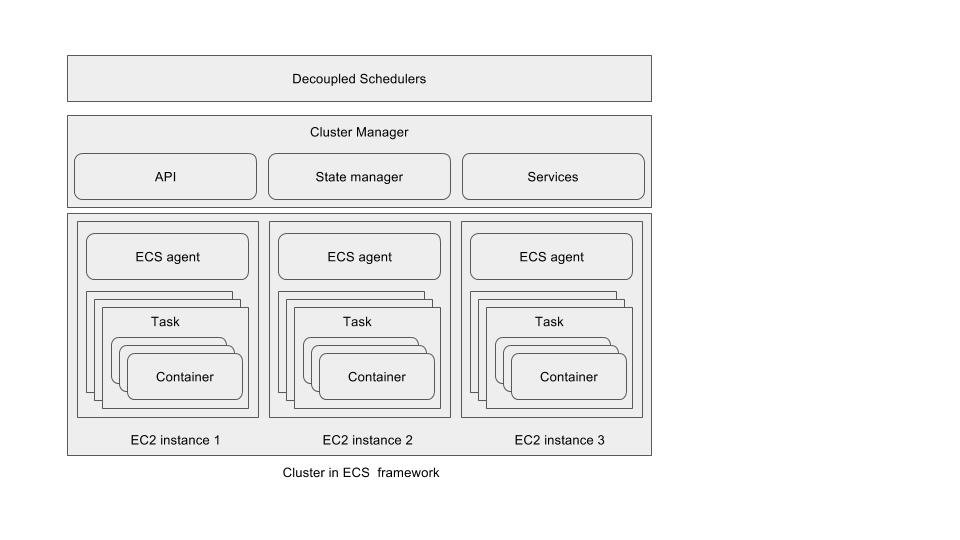
\includegraphics[scale=0.5]{./fig/ecs}
\caption{Amazon ECS Architecture}
\label{fig:ecsArch}
\end{figure*}

Amazon EC2 instances are virtual computing environment created by using the configuration template called Amazon Machine Image (AMI). AMI is preconfigured template which contains all the configuration details like services, kernel, application details etc. User can create his own image instead of using AMI. 

The instances of AMI are just like a host machine which are used to launch and deploy the applications quickly. More than one instances of a single AMI can be launched with different types. Type of the instance is used to determine the physical configuration of the host machine where the instance will be running. In case of failure of an instance, a new instance can be launched using the AMI template.

Amazon ECS has three tasks: Cluster Management Engine, state management and back-end services. Scheduler is decoupled from the cluster manager which allows the user to have their own scheduler making the scheduler as a plug-in. In ECS framework, cluster consists of a collection of EC2 instances. Each of these EC2 instances runs multiple containers. To coordinate with these EC2 instances, ECS cluster manager talks to a daemon, called ECS agent, which runs on each of these EC2 instances. ECS agents allows the ECS manager to launch, deploy and monitor the containers as per the default or the scheduler given by the user.

To coordinate with the cluster, ECS stores and maintains the cluster state information. Cluster state is stored in key/value pair. To be scalable and to avoid network or hardware failure, this key/value is distributed across the cluster. ECS uses Amazon’s core distributed system mechanism, called Paxos-based transactional journal based data store, to handle the concurrent changes in the key/value data.

ECS’s distributed cluster systems is more robust as it takes away the need to setup, run and administer the orchestration layer. 

Service discovery is not provided by ECS. You have to do the service discovery using a third party tool e.g. Zookeeper.

Following are the features of EC2 Container Service:

\begin{enumerate}
\item Compatibility with Docker containers:
ECS uses Docker containers to schedule the services and applications on the cluster of EC2 instances. Each of the EC2 instances has a Docker daemon running on them to run the container scheduled by ECS. EC2 is limited to Docker containers and not compatible with any other container platform.

\item Flexible Scheduling:
Built in scheduler of ECS will distribute the containers across the cluster to balance the requirement and availability of the resources. Decoupling of scheduler from cluster manager enables the user to integrate and use their own scheduler.

\item Task Definitions:
Task Definition is a JSON template which is used by ECS to define the tasks. Task Definition allows us to specify the requirements related to Docker image and hardware. It also allows to specify if the containers are related to each other. Multiple tasks can be launched from one task definition file. We can also have version control of the application using task definition file.

\item Scalability with high performance:
Thousands of containers can be started, stopped and managed within seconds.

\item Amazon Web Service Integration:
ECS is designed to allow the application to use other AWS features like features such as Elastic IP addresses, resource tags, IAM, CloudTrail and Virtual Private Cloud (VPC).

\end{enumerate}

In the following section, we have discussed and provided comparison of the various features of these five container orchestration tools.
\input{sysdesc}
\input{design}
\input{issues}
\input{approach}
\input{related}


\input{evaluation}
\section{Comparative Study of Container Management Tools}
\label{sec:comparison}
The tools  discussed in this paper supports most of the basic features of a container orchestration tools. However, these tools differ from each other by supporting additional other features, in terms of their compatibility, easy of use and extensibility. 

Apache's Mesos has  been used in large production environment supporting tens of thousands of nodes. It is designed for big clusters. Hence, it is complicated to use Mesos in a small cluster. However, CoreOS's Fleet limitation to hundreds of nodes makes it more suitable for small scale cluster. With recent development, Kubernetes and Docker's Swarm supports a cluster of thousand nodes too. 

Due to built on the several years of experience in production environment, Kubernetes is most versatile in terms of various functionalities. For example, it supports smooth rolling update with feature to rollback. With its labeling feature, it is easy to group the task. Kubernetes is also supported by many PaaS tools. Apart from Kubernetes, Swarm also supports labeling. Swarm allows tagging a node with multiple labels which allows user to put multiple and wider constraints on a container.

Service discovery feature is supported by all the discussed tools. However, Amazon's ECS requires Docker's native container link functionality to support service discovery. 

The other two basic features of a container orchestration tool, state management and scheduling, is supported by all the discussed tools.  Mesos, Swarm and ECS allow to have a third party scheduler separating the scheduling from the state management, while Kubernetes and Fleet doesn't.

Kubernetes and Mesos are the only ones that support health monitoring. This feature is made easier by Amazon's ECS because ECS handles the health monitoring itself making it automated.

High availability of the master node is only supported by Mesos, Swarm and Fleet since they allow to have multiple instances of the master node. Kubernetes and ECS doesn't have multiple instances of master node, so they don't support high availability.

CoreOS's Fleet uses etcd and extends the systemmd feature, which was designed for single host, to support a multiple nodes cluster. In Fleet's framework, each node runs fleet daemon so any node can be a master node. So, instead of having multiple instances of master nodes, fleet implements distributed master node. 

Since Fleet is a lower level software, handling all the features is not as smooth compared to other tools for example: scheduling based on utilization. It is more suitable to run another orchestration tool on top of CoreOS's Fleet.

Mesos, fleet and ECS allows to run other orchestration tools on top of them. For example, we can run kubernetes on top of coreOs's fleet. However, Kubernetes and Swarm doesn't support this feature.

Feature of having a persistent data on a node which is shared across the containers is supported by all the mentioned tools.

In terms of ease of use, Docker's Swarm is on the top due to its compatibility with Docker's API. Containers can launched with simple Docker command. Being the native tool of a Docker, it is easily compatible with other Docker tools. However, any limitation of Docker APIs are obviously the limitations of Docker's Swarm.

Docker Swarm is also very lightweight compared to other tools except CoreOS's fleet which is a lightweight linux distribution without having any package manager. The requirement to prescale the cluster in Amazon's ECS is its only disadvantage in terms of easy of use.

Except for Swarm, container's recovery is supported by kubernetes, Mesos and ECS.

To summarize, all these tools supports the basic features of a container orchestration tool. While Docker's Swarm compatibility with Docker's API makes it easier to use, Kubernetes's robustness and making the faults not affecting availability is well tested as Kubernetes is based on 15 years of experience in production environment. Being lower level software, CoreOS's Fleet is more suitable for a small cluster and running other tools on top of it. If your application or services are already using AWS features, Amazon's ECS is the best choice. Although Mesos was developed before the sudden growth in use of containers, it supports cluster of containerized applications and if the cluster has tens of thousands of nodes, then Mesos is the best choice.

Table 1 summarizes the comparison of various features of these five container management tools discussed in this section.

\begin{figure*}
\centering
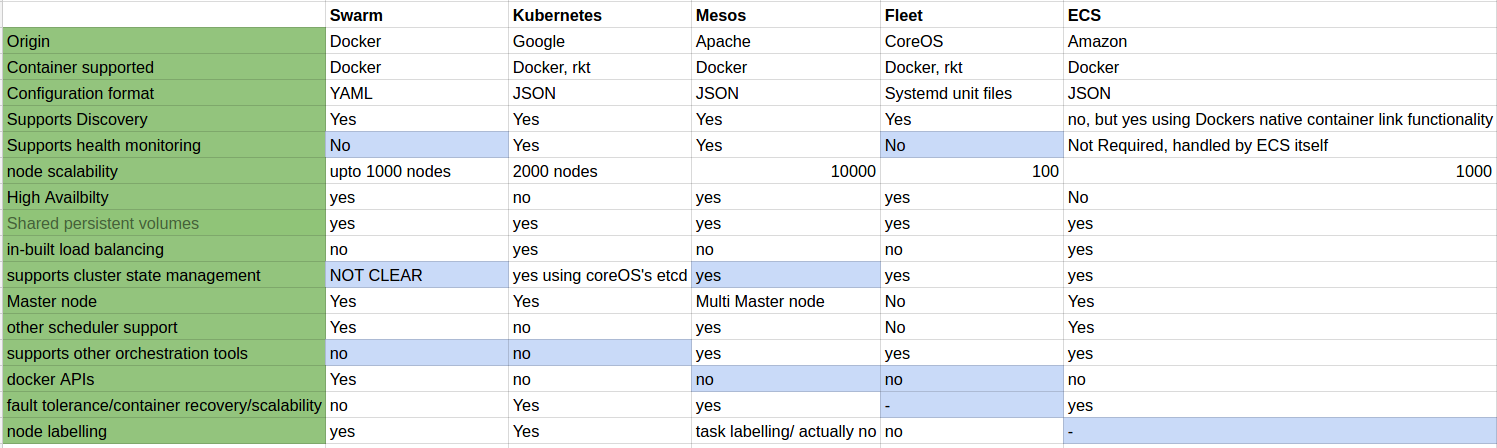
\includegraphics[width=\textwidth]{./fig/comparison}
\caption{Comparison Table}
\label{fig:comparison}
\end{figure*}


\begin{table*}[ht]
\caption{Comparison of various features}
\centering
\begin{tabular}{p{0.14\linewidth}p{0.14\linewidth}p{0.14\linewidth}p{0.14\linewidth}p{0.14\linewidth}p{0.14\linewidth}}
\hline
Features & Swarm & Kubernetes & Mesos & Fleet & ECS\\
\hline
Origin & Docker & Google & Apache &	CoreOS & Amazon\\

Container supported & Docker & Docker, rkt & Docker &	Docker, rkt & Docker\\

Configuration format	& YAML &	JSON & JSON & Systemd unit files & JSON\\

Supports Discovery  & yes & yes & yes & yes & no\raise0.5ex\hbox{1}\\

Supports health monitoring & no & yes & yes & no & no\raise0.5ex\hbox{2}\\

node scalability	& upto 1000 nodes & 2000 nodes & 10000 & 100 & 1000\\

High Availbilty	& yes &	no & yes &	yes &	no\\

Shared persistent volumes & yes & yes & yes & yes & yes\\

in-built load balancing & no &	yes &	no &	no &	yes\\

supports cluster state management & NOT CLEAR & yes\raise0.5ex\hbox{3} & yes & yes & yes\\

Master node	 & yes & yes & Multi Master node &	no &	yes\\

other scheduler support & yes & no & yes & no & Yes\\

supports other orchestration tools	 & no  & no &	yes &	yes &	yes\\

docker APIs	 & yes & no &	no & no & no\\

fault tolerance/container recovery/scalability  & no & yes & yes & - & yes\\

node labelling & yes & yes & no\raise0.5ex\hbox{4} & no & -\\
\hline
\end{tabular}
\\
1. yes, using Dockers native container link functionality\\
2. Not required as it is handled by ECS itself\\
3. using coreOS's etcd\\
4. But task labelling: yes
\end{table*}


\section{Open Issues and approach}
\label{sec:OIA}

In a cluster of containers, monolithic services and large applications are broken down into micro-services and smaller applications to improve the resource utilizations and workload sharing.
It is not so easy to disintegrate a monolithic service or application due to the complexity involved in the business processes using those services. In production environment, millions of containers are started every day on a cluster of thousands of hosts, for an instance: Kubernetes claims to launch billions of containers every week. With the recent advancement in container orchestration tools, managing and scheduling so many containerized applications on a cluster has become convenient. However, deploying millions of containers on thousands of hosts on a cluster has multiple failure points e.g. out-of memory issue or network failure. This also includes failure of a running host. Due to these failure points, challenges related to horizontal scaling of the containers and maximizing the resource utilization remain open. 

Dockers indicate that the maximum number of containers running on a host is roughly 600 (needs reference) which makes the need of horizontal scaling of containers necessary. 

The challenge is to make the horizontal scaling effective utilizing the resources efficiently. To utilize the resources effectively, bin-packing is used to containerize applications. bin-packing decision is a np-complete problem. Since the applications running in a container can be long jobs or batch jobs, it becomes even harder to make the decision on the resources. Additionally, it is also possible that an already scheduled job, e.g. weekly scheduled Spark batch job, is hogging the resources even though it is not using them starving the other applications from the resources. 

Scaling of containers may cause resource segmentation (??????? this is my term based on my understanding so far, i am not sure if it is the right term ???????)

To solve these issues, we propose to have containers shared across the nodes in a cluster i.e. running a container on two hosts at the same time. Implementing a shared container will make the resource utilization hard and dynamic. A shared container will run on multiple hosts with its own limit of resources on each of the hosts. The shared container will have a net limit on the resource utilization which will be sum of its individual limitations for each hosts. For instance, a shared container is running on machine A and machine B. It will have its own memory, CPU etc limit for machine A and machine B separately. The total limit of the container will be equal to its limit set on machine A and machine B. 

In case, the container is reaching its limit set for machine A and its usage on machine B is still under the limit, then we can adjust the limit of the container on machine A by increasing it if the resources are available on machine A. This will of-course result in decreasing its resource limit for machine B.  However, the overall limit will still stay the same.

By adjusting the container limits by sharing it on multiple nodes, we will make sure the resource utilization are dynamic and efficient. 

Sharing the containers on multiple nodes may also solve the issue of container failure. If the container fails on one machine, it can be recovered on another machine if the resources are available instead of recovering it from its instances. This way we don't need to have multiple instances of the containers.


We can talk about the applications and usage of this solutions: I am not sure if we should talk about its application for e.g. sharing workload of mobile phone on cloudlets.
\section{Conclusion}
\label{sec:conclusion}
conclusion goes here

% use section* for acknowledgment
%\section*{Acknowledgment}



\bibliographystyle{plain}
\bibliography{common}


%\begin{thebibliography}{1}
%\bibitem{Referred Name}
%author 1 and author 2: "The title of the paper". \emph{In Proceedings of XYCZ}, \relax (conference name year), [Online] Month Year.
%\end{thebibliography}



% that's all folks
\end{document}


